\documentclass[border=4pt]{standalone}
\usepackage{tikz}
\usepackage{pgfplots}
\pgfplotsset{compat=1.18}
\usetikzlibrary{shapes.geometric,arrows.meta,positioning,calc,fit,decorations.pathreplacing,backgrounds}
\definecolor{boxblue}{RGB}{225,238,252}
\definecolor{boxgreen}{RGB}{225,247,231}
\definecolor{boxorange}{RGB}{253,236,216}
\definecolor{boxgray}{RGB}{237,237,237}
\definecolor{boxred}{RGB}{253,226,226}
\begin{document}
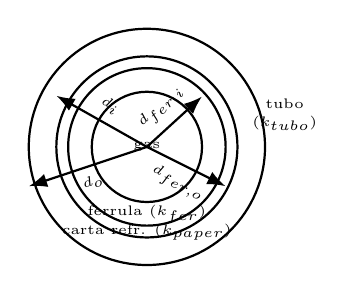
\begin{tikzpicture}
\fill[boxblue] (0,0) circle (0.7);
\fill[boxgray] (0,0) circle (1.0) circle (0.7);
\fill[boxorange] (0,0) circle (1.15) circle (1.0);
\fill[white] (0,0) circle (1.5) circle (1.15);
\draw[thick] (0,0) circle (0.7);
\draw[thick] (0,0) circle (1.0);
\draw[thick] (0,0) circle (1.15);
\draw[thick] (0,0) circle (1.5);
\node[font=\tiny] at (0,0) {gas};
\node[font=\tiny,align=center] at (1.75,0.55) {tubo};
\node[font=\tiny,align=center] at (1.75,0.3) {($k_{tubo}$)};
\draw[-{Latex},thick] (0,0) -- (0.7,0.64) node[midway,above,sloped,font=\tiny]{$d_{fer,i}$};
\draw[-{Latex},thick] (0,0) -- (1.0,-0.5) node[midway,below,sloped,font=\tiny]{$d_{fer,o}$};
\draw[-{Latex},thick] (0,0) -- (-1.15,0.65) node[midway,above,sloped,font=\tiny]{$d_i$};
\draw[-{Latex},thick] (0,0) -- (-1.5,-0.5) node[midway,below,sloped,font=\tiny]{$d_o$};
\node[font=\tiny] at (0,-0.85) {ferrula ($k_{fer}$)};
\node[font=\tiny] at (0,-1.08) {carta refr. ($k_{paper}$)};
\end{tikzpicture}
\end{document}
